\documentclass[10pt,a4paper]{article}
\usepackage[utf8]{inputenc}
\usepackage[T1]{fontenc}
\usepackage{lmodern}
\usepackage[english]{babel}
\usepackage[margin=2.1cm]{geometry}
\usepackage{amsmath,amssymb,mathtools,bm}
\usepackage{booktabs,array,tabularx}
\newcolumntype{L}[1]{>{\raggedright\arraybackslash}p{#1}}
\newcolumntype{Y}{>{\raggedright\arraybackslash}X}
\usepackage{graphicx}
\usepackage{float}
\usepackage[font=small]{caption}
\usepackage{xcolor}
\usepackage{tikz}
\usetikzlibrary{calc,arrows.meta,positioning}
\usepackage[hidelinks]{hyperref}
\usepackage{url}
\numberwithin{equation}{section}
\setlength{\emergencystretch}{3em}
\newcommand{\note}[1]{\begin{center}\fcolorbox{red!70!black}{red!5}{\parbox{0.94\linewidth}{\small\textbf{Note.} #1}}\end{center}}
\newcommand{\KppAzEst}{7.43}
\newcommand{\KppElEst}{8.57}
\newcommand{\KpvAzEst}{198}
\newcommand{\KpvElEst}{61}
\newcommand{\KivAzEst}{0.15}
\newcommand{\KivElEst}{0.73}
\newcommand{\TcAzEst}{0.30}
\newcommand{\TcElEst}{0.29}
\newcommand{\TcAzHsix}{1.58}
\newcommand{\TcElHsix}{0.66}
\newcommand{\SepFitAzEst}{93}
\newcommand{\SepFitElEst}{84}
\newcommand{\OctFitAzA}{11}
\newcommand{\OctCurAzA}{-108}
\newcommand{\OctFitElA}{-9}
\newcommand{\OctCurElA}{9}
\newcommand{\OctFitAzB}{76}
\newcommand{\OctCurAzB}{-127}
\newcommand{\OctFitElB}{-275}
\newcommand{\OctCurElB}{-13}
\newcommand{\OctFitAzC}{-1}
\newcommand{\OctCurAzC}{-114}
\newcommand{\OctFitElC}{-24}
\newcommand{\OctCurElC}{-269}
\newcommand{\OctFitAzD}{32}
\newcommand{\OctCurAzD}{-135}
\newcommand{\OctFitElD}{-15}
\newcommand{\OctCurElD}{-207}
\newcommand{\OctFitAzE}{-12}
\newcommand{\OctCurAzE}{-165}
\newcommand{\OctFitElE}{-3}
\newcommand{\OctCurElE}{44}
\newcommand{\OctFitAzF}{69}
\newcommand{\OctCurAzF}{5}
\newcommand{\OctFitElF}{-259}
\newcommand{\OctCurElF}{9}
\newcommand{\OctFitAzG}{83}
\newcommand{\OctCurAzG}{19}
\newcommand{\OctFitElG}{47}
\newcommand{\OctCurElG}{-125}
\newcommand{\OctFitAzH}{77}
\newcommand{\OctCurAzH}{22}
\newcommand{\OctFitElH}{91}
\newcommand{\OctCurElH}{49}
\newcommand{\CtrlErrDb}{0.001}
\newcommand{\CtrlErrDeg}{0.25}
\newcommand{\LinCheck}{5e-09}
\newcommand{\NmovesOctAz}{12}
\newcommand{\NmovesOctEl}{14}


\title{Closed-loop model of the LUCY mount:\\ comparison with the time sequences and the step tests}
\author{Generated by \texttt{build\_closed\_loop\_report.py}\\ \small\texttt{sim/gimbal\_multidof/closedLoopModel/report}}
\date{\today}
\begin{document}
\maketitle

\paragraph{Purpose.} This report compares the closed-loop model of the mount (mechanics, motors and drives) with the measurements taken on LUCY. There are two sets of data:
\begin{itemize}
\item the time sequences recorded in September (\texttt{LucyIdentification/Validation});
\item the frequency responses and the step tests of October (\texttt{LucyIdentification/VClosedLoop}).
\end{itemize}
The report explains the context built for the comparison (Sections~\ref{sec:model}--\ref{sec:method}), the configurations that were tested and why they were needed (Sections~\ref{sec:sep}--\ref{sec:oct}), the results, and what remains open (Section~\ref{sec:concl}).

\paragraph{Main results.}
\begin{itemize}
\item \textbf{Azimuth.} The drive parameters of the files reproduce the step tests only if the position gain \texttt{PL.KP} is read in 1/s (median fit of the position error \OctFitAzB\,\%). Read in Hz, as WorkBench does in its Controller trace, the fit is \OctFitAzA\,\%. Both test campaigns agree on this.
\item \textbf{Elevation.} No reading of the parameters of the files reproduces the tests (fit at most \OctFitElE\,\%). The gains estimated on the September sequences predict the October tests with a median fit of \OctFitElH\,\%: the elevation drive behaves consistently between the two campaigns, but not as its parameter file says.
\item \textbf{Feedforward.} The velocity feedforward written in the files (\texttt{VL.KVFF} $=1$) always makes the comparison worse: it is not active in the tests.
\item \textbf{Friction.} The Coulomb friction of the bearings during the moves is about 0.3\,N\,m on both axes. This is 2--5 times less than the Dahl element derived from the H6 frequency responses.
\item \textbf{Model limits.} The coupling between the axes is underestimated by one to two orders of magnitude, a current oscillation at 8--10\,Hz is not reproduced, and the low-frequency response of the azimuth is not repeatable between tests.
\end{itemize}

\tableofcontents

%% ===================================================================================================
\section{The closed-loop model}\label{sec:model}
The model is the library \texttt{lucy\_cl} in \texttt{sim/gimbal\_multidof/closedLoopModel}. It has three independent components connected in a closed loop for each axis (Figure~\ref{fig:loop}).
\begin{itemize}
\item \textbf{Mechanical plant:} the nonlinear 8-DOF lumped model H6 of \texttt{gimbal\_mdof}, with all the Newton--Euler terms. Its coordinates are $\mathbf q=[\psi_e,\psi_m,\psi_L,\theta_e,\theta_h,\theta_m,\theta_r,\theta_p]$: encoder, motor and fork nodes of the azimuth; encoder, hub, motor, ring and telescope nodes of the elevation. Any other configuration of \texttt{gimbal\_mdof} can replace it.
\item \textbf{Motors:} two Kollmorgen TBM(S)-7646-A frameless motors with datasheet parameters. The model is a per-phase rms model of the $q$-axis current,
\begin{equation}
L_{ph}\,\frac{di}{dt}=v-R_{ph}\,i-\frac{K_b}{\sqrt3}\,\omega_m,\qquad \tau_m=K_t\,i-b_m\,\omega_m ,
\end{equation}
with $K_t=0.258$\,N\,m/A$_\mathrm{rms}$ at 25\,$^\circ$C, which equals $\sqrt3\,K_b$ to within 0.01\,\%. The rotor inertia is added to the motor node of the plant.
\item \textbf{Drives:} Kollmorgen AKD2G in position mode. The drive model is a cascade of three loops:
  \begin{itemize}
  \item a position loop $v_{cmd}=K_{pp}(p_{cmd}-p_{fb})$;
  \item a velocity loop $i_{cmd}=K_{pv}(1+2\pi K_{iv}/s)\,H_{AR1}H_{AR2}\,(v_{cmd}-H_{AR3}H_{AR4}H_{obs}\,v_{fb})$, with the biquad filters AR1--AR4 and the observer modelled as a first-order low pass;
  \item a current PI with its zero on $R/L$ (crossover 1.5\,kHz).
  \end{itemize}
  The limits are the current limit (\texttt{IL.LIMITP} $=18$\,A), the clamp of the velocity integrator and the bus voltage (34\,V). Anti-windup is by back-calculation.
\end{itemize}
\begin{figure}[H]\centering
\resizebox{\linewidth}{!}{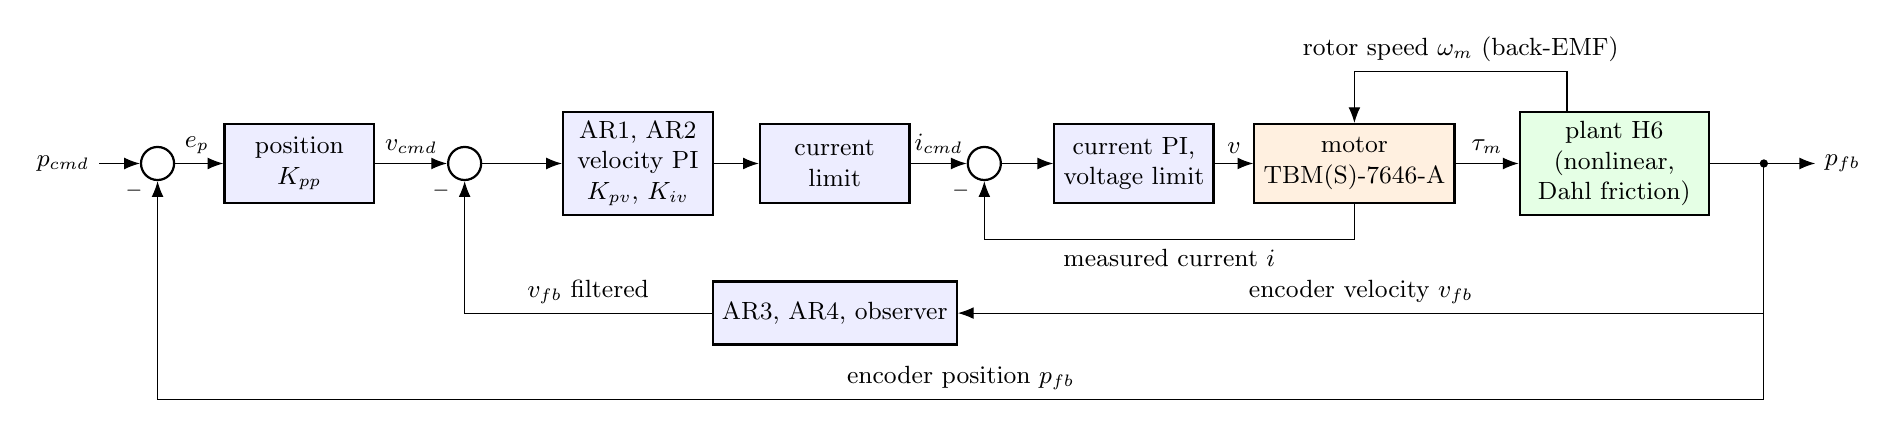
\begin{tikzpicture}[font=\small, >={Latex[length=2mm]},
 blk/.style={draw, thick, fill=blue!7, minimum height=1.0cm, minimum width=1.9cm, align=center},
 sum/.style={draw, thick, circle, inner sep=0pt, minimum size=0.42cm}]
\node (pc) at (0,0) {$p_{cmd}$};
\node[sum] (s1) at (1.2,0) {};
\node[blk] (pl) at (3.0,0) {position\\ $K_{pp}$};
\node[sum] (s2) at (5.1,0) {};
\node[blk] (vl) at (7.3,0) {AR1, AR2\\ velocity PI\\ $K_{pv}$, $K_{iv}$};
\node[blk] (lim) at (9.8,0) {current\\ limit};
\node[sum] (s3) at (11.7,0) {};
\node[blk] (il) at (13.6,0) {current PI,\\ voltage limit};
\node[blk, fill=orange!12] (mot) at (16.4,0) {motor\\ TBM(S)-7646-A};
\node[blk, fill=green!10, minimum width=2.4cm] (pla) at (19.7,0) {plant H6\\ (nonlinear,\\ Dahl friction)};
\node (out) at (22.6,0) {$p_{fb}$};
\coordinate (tap) at (21.6,0);
\draw[->] (pc) -- (s1); \draw[->] (s1) -- node[above, pos=0.45] {$e_p$} (pl);
\draw[->] (pl) -- node[above] {$v_{cmd}$} (s2);
\draw[->] (s2) -- (vl); \draw[->] (vl) -- (lim); \draw[->] (lim) -- node[above] {$i_{cmd}$} (s3);
\draw[->] (s3) -- (il); \draw[->] (il) -- node[above] {$v$} (mot); \draw[->] (mot) -- node[above] {$\tau_m$} (pla);
\draw[->] (pla) -- (out);
% current feedback
\draw[->] (mot.south) -- ++(0,-0.45) -| node[pos=0.25, below] {measured current $i$} (s3.south);
% back-EMF
\draw[->] ([xshift=-0.6cm]pla.north) -- ++(0,0.5) -| node[pos=0.25, above] {rotor speed $\omega_m$ (back-EMF)} (mot.north);
% velocity feedback
\node[blk, minimum width=2.2cm, minimum height=0.8cm] (fb) at (9.8,-1.9) {AR3, AR4, observer};
\draw[->] (tap) -- (21.6,-1.9) -- node[above, pos=0.5] {encoder velocity $v_{fb}$} (fb.east);
\draw[->] (fb.west) -| node[pos=0.25, above] {$v_{fb}$ filtered} (s2.south);
% position feedback
\draw[->] (tap) -- (21.6,-3.0) -| node[pos=0.25, above] {encoder position $p_{fb}$} (s1.south);
\fill (tap) circle (1.5pt);
\node at (0.9,-0.35) {\scriptsize $-$}; \node at (4.8,-0.35) {\scriptsize $-$}; \node at (11.4,-0.35) {\scriptsize $-$};
\end{tikzpicture}}
\caption{Closed loop of one axis in the model. The drive acts on the measured current and the motor on the applied voltage, so there is no algebraic loop. The feedback is the load-side encoder.}\label{fig:loop}
\end{figure}

\paragraph{Assumptions specific to the comparison.}
\begin{itemize}
\item \textbf{Telescope balanced}, $g=0$. The CAD places the centre of gravity 73\,mm from the polar axis, which would give 11\,N\,m of gravity moment. The motor gives only 4.6\,N\,m at the current limit, and the holding torques measured at rest do not depend on the elevation angle (Section~\ref{sec:sep}).
\item \textbf{Bearing friction.} In the time domain it is a Dahl element on the bearing node,
\begin{equation}
\dot T_f=\sigma_0\bigl(\dot q-|\dot q|\,T_f/T_c\bigr),
\end{equation}
calibrated so that, at the amplitude of the frequency-response test, its describing function equals the H6 ground constraint $k(1+j\eta)$. The H6 values are $T_c=\TcAzHsix$\,N\,m (azimuth) and \TcElHsix\,N\,m (elevation).
\item \textbf{Damping of the plant.} H6 as identified uses the placeholder damping $\zeta_1=0.01$ (Q8 of \texttt{gimbal\_mdof}). With it the elevation loop is unstable at about 300\,Hz (Table~\ref{tab:zeta}, Figure~\ref{fig:zeta}): the mode of the hub and motor side against the telescope on $k_b$ is too lightly damped, while the measured loop is stable with 17\,dB of gain margin. All the time simulations therefore use $\zeta_1=0.10$, a sensitivity value and not an identified one.
\end{itemize}
\begin{table}[H]\centering\small
\caption{Damping sensitivity (October drive parameters, position gain $2\pi$\,\texttt{PL.KP}): phase margin [deg] / smallest gain margin [dB] at frequency [Hz] of the loop at the current command, and largest real part of the closed-loop eigenvalues of the linearised time model [1/s].}\label{tab:zeta}
\begin{tabular}{llll}\toprule
$\zeta_1$ & azimuth & elevation & max Re(eig) [1/s] \\ \midrule
0.01 & 25 / 20.3 at 1605 & -18 / -5.8 at 300 & 35 \\
0.02 & 25 / 25.1 at 1572 & -7 / -1.5 at 304 & 17.7 \\
0.05 & 25 / 30.7 at 1515 & 59 / 4.0 at 312 & 2.65e-13 \\
0.1 & 25 / 34.7 at 1496 & 59 / 8.6 at 319 & -4.01e-14 \\
0.2 & 25 / 40.4 at 1625 & 59 / 15.1 at 327 & 4.3e-13
\\ \bottomrule
\end{tabular}\end{table}
\begin{figure}[H]\centering
\includegraphics[width=0.66\linewidth]{figures/fig_zeta}
\caption{Elevation loop at the current command for three values of $\zeta_1$. With $\zeta_1=0.01$ the magnitude exceeds 0\,dB near 300\,Hz, where the phase crosses $-180^\circ$. The gain margin is then negative ($-5.8$\,dB) and the loop is unstable.}\label{fig:zeta}
\end{figure}

\paragraph{Checks of the implementation.}
\begin{itemize}
\item The model of the drive reproduces the ``Controller'' trace of every WorkBench export to \CtrlErrDb\,dB and \CtrlErrDeg$^\circ$ over 1--2000\,Hz (Figure~\ref{fig:controller}). The ``Feedback Biquad'' trace is reproduced too. WorkBench computes its Open Loop as Controller $\times$ Plant $\times$ Feedback Biquad and its Closed Loop as Controller $\times$ Plant$/(1+$Open Loop$)$; both relations were checked to machine precision.
\item The time-domain model linearised by finite differences coincides with the frequency-domain model to a relative difference of \LinCheck.
\end{itemize}
\begin{figure}[H]\centering
\includegraphics[width=0.92\linewidth]{figures/fig_controller}
\caption{Controller trace (velocity feedback to current command, position loop included) of the October WorkBench exports, against the model of the drive built from the parameters of the test.}\label{fig:controller}
\end{figure}

%% ===================================================================================================
\section{Measurements}\label{sec:data}
\begin{table}[H]\centering\small
\caption{Time sequences: campaign, file, duration [s], number of moves (azimuth / elevation), amplitudes of the moves [deg], use. The September files \texttt{Position\_dist\_FF*.csv} are not used, at the user's request.}\label{tab:seq}
\begin{tabularx}{\linewidth}{llrrlY}\toprule
campaign & sequence & duration & moves & amplitudes & use \\ \midrule
Sept. & \texttt{MPCLucy\_pos\_dist\_dataset} & 100 & 4 / 21 & 1, 10 & estimate of the effective gains \\
Sept. & \texttt{MPCLucy\_pos\_dist\_test} & 100 & 1 / 23 & 1, 2, 10 & validation \\
Sept. & \texttt{MPCLucy\_scotched} & 100 & 11 / 11 & 2, 3, 10, 20 & validation \\
Oct. & \texttt{MPCLucy\_step\_1deg} & 26 & 4 / 6 & 0.6, 1 & comparison with the parameters of the files \\
Oct. & \texttt{MPCLucy\_1degAz\_zeroAz\_1degPol\_\_zeroPol} & 66 & 4 / 4 & 1 & comparison with the parameters of the files \\
Oct. & \texttt{MPCLucy\_2degAz\_2degPol\_zeroAz\_zeroPol} & 50 & 2 / 2 & 2 & comparison with the parameters of the files \\
Oct. & \texttt{MPCLucy\_2degPol\_zeroPol\_2degAz\_zeroAz} & 31 & 2 / 2 & 2 & comparison with the parameters of the files
\\ \bottomrule
\end{tabularx}\end{table}
The sequences are sampled at 2\,kHz. For both axes they contain:
\begin{itemize}
\item the command position and the encoder position, in millidegrees (360\,000 units per revolution, encoder step 0.343\,mdeg);
\item the current channel \texttt{AXIS*\_AMPS};
\item the torque channel \texttt{AXIS*\_TORQUE} estimated by the drives.
\end{itemize}
\texttt{AXIS1} is the azimuth and \texttt{AXIS2} the elevation. The commands are trapezoidal speed profiles: 15\,deg/s and 200\,deg/s$^2$ in September, 10\,deg/s in October. The October campaign also contains two frequency responses (one per axis) and the drive parameter files active during the tests (Table~\ref{tab:files}).

\paragraph{Scale of the current channel.} \texttt{AXIS*\_AMPS} saturates at 35.9, twice the current limit of the drives (18\,A$_\mathrm{rms}$). The rigid-body balance of the moves confirms the scale (Figure~\ref{fig:scale}, Table~\ref{tab:scale}). On the encoder and current signals low-passed at 3\,Hz,
\begin{equation}
\mathrm{AMPS}=a\,\ddot q+b\,\mathrm{sgn}\,\dot q+c .
\end{equation}
With the rigid inertias of the model, $J/a$ is the torque per unit of the channel. It is 0.13--0.15\,N\,m, that is about $K_t/2$. One unit is therefore taken as 0.5\,A$_\mathrm{rms}$, a choice the user confirmed. The torque channel of the files is $0.1847\times$AMPS, which is 1.4 times this value. The same regression gives the Coulomb friction during the moves: 0.3--0.4\,N\,m.
\begin{figure}[H]\centering
\includegraphics[width=0.95\linewidth]{figures/fig_current_scale}
\caption{Current channel against the encoder acceleration during the moves of \texttt{MPCLucy\_pos\_dist\_dataset}, separated by the sign of the speed. The parallel lines are $a\ddot q\pm b+c$; their vertical distance $2b$ is twice the Coulomb friction.}\label{fig:scale}
\end{figure}
\begin{table}[H]\centering\small
\caption{Rigid-body balance of the moves: slope $a$ [units/(rad/s$^2$)], torque per unit $J/a$ [N\,m], torque per A$_\mathrm{rms}$ with 2 units per ampere [N\,m/A] (datasheet $K_t=0.258$), Coulomb friction [N\,m], coefficient of determination.}\label{tab:scale}
\begin{tabular}{llrrrrr}\toprule
sequence & axis & $a$ & $J/a$ & $2J/a$ & Coulomb & $R^2$ \\ \midrule
\texttt{MPCLucy\_pos\_dist\_dataset} & azimuth & 16.29 & 0.132 & 0.264 & 0.30 & 0.994 \\
\texttt{MPCLucy\_pos\_dist\_dataset} & elevation & 5.97 & 0.151 & 0.302 & 0.40 & 0.972 \\
\texttt{MPCLucy\_pos\_dist\_test} & azimuth & 15.57 & 0.138 & 0.277 & 0.07 & 0.996 \\
\texttt{MPCLucy\_pos\_dist\_test} & elevation & 6.13 & 0.147 & 0.294 & 0.36 & 0.964 \\
\texttt{MPCLucy\_scotched} & azimuth & 16.71 & 0.129 & 0.258 & 0.31 & 0.993 \\
\texttt{MPCLucy\_scotched} & elevation & 6.24 & 0.144 & 0.289 & 0.36 & 0.976
\\ \bottomrule
\end{tabular}\end{table}
\begin{table}[H]\centering\small
\caption{Drive parameters in the files: September (\texttt{Validation/*\_Parameters.akd}) and October (\texttt{VClosedLoop/Parameters\_*.akd}).}\label{tab:files}
\begin{tabularx}{\linewidth}{lYYYY}\toprule
 & azimuth, Sept. & azimuth, Oct. & elevation, Sept. & elevation, Oct. \\ \midrule
PL.KP & 10 & 10 & 0.4 & 0.4 \\
PL.KI & 0 & 0 & 0 & 0 \\
VL.KP [A/(rad/s)] & 250 & 250 & 30 & 25 \\
VL.KI [Hz] & 1 & 1 & 20 & 15 \\
VL.KVFF & 1 & 1 & 1 & 1 \\
observer (OBS.ENABLE) & 0 & 0 & 1 & 1 \\
IL.LIMITP [A rms] & 18 & 18 & 18 & 18 \\
active biquads & AR1: 65\,Hz, +10\,dB; AR2: 500/14\,Hz & AR1: 65\,Hz, +10\,dB; AR2: 500/14\,Hz & AR3: 5000/800\,Hz; AR4: 5000/800\,Hz & AR1: 50\,Hz, -12\,dB; AR2: 96\,Hz, -12\,dB; AR3: 5000/800\,Hz; AR4: 5000/800\,Hz
\\ \bottomrule
\end{tabularx}\end{table}

%% ===================================================================================================
\section{Comparison method}\label{sec:method}
Every move is simulated separately, in a window that starts 0.3\,s before the move and ends 2.5\,s after it (or just before the next move of either axis). The model starts from the state measured at rest before the move:
\begin{itemize}
\item the encoder positions of both axes;
\item the holding currents, carried by the friction state and clipped below $T_c$;
\item the static twist of the shafts under that torque;
\item integrators consistent with it.
\end{itemize}
It is then driven by the measured commands of both axes. Two signals of the moving axis are compared, the position error $e=p_{cmd}-p_{enc}$ and the current, together with the error of the held axis.

The goodness of fit is the NRMSE fit of the System Identification Toolbox:
\begin{equation}
\mathrm{fit}=100\left(1-\frac{\lVert y-\hat y\rVert}{\lVert y-\bar y\rVert}\right)\ \%.
\end{equation}
100 is a perfect model, 0 is no better than the mean of the measurement, and the value can be negative.

The integration uses an implicit solver (Radau) on the whole nonlinear loop; the encoder nodes are very stiff. A window of 3\,s takes 2--4\,s of computation.

%% ===================================================================================================
\section{September sequences: why the drive gains had to be estimated}\label{sec:sep}
\paragraph{The parameters of the files do not reproduce the sequences.} At constant commanded speed the following error of a proportional position loop is $e=v/K_{pp}$. At 15\,deg/s, the files read as WorkBench reads them ($K_{pp}=2\pi\,$\texttt{PL.KP}) give:
\begin{itemize}
\item 0.24\,deg on the azimuth ($K_{pp}=62.8$\,1/s);
\item 6\,deg on the elevation ($K_{pp}=2.5$\,1/s).
\end{itemize}
Both axes show instead about 2\,deg. The azimuth gains differ from the elevation gains by a factor of 25, yet the two axes have the same error, which no reading of the files explains. The simulations confirm it (red curves in Figure~\ref{fig:sepmoves}):
\begin{itemize}
\item the azimuth overshoots by 1\,deg with the current saturated, while the measurement is slow and well damped;
\item the elevation lags by up to 4\,deg.
\end{itemize}
The drive configuration active during the sequences was not available. The elevation file is dated 11 September and the sequences 14--21 September. The user therefore chose to estimate the effective gains from the data.

\paragraph{Estimate.} Four parameters per axis are estimated on the moves of \texttt{MPCLucy\_pos\_dist\_dataset}: $K_{pp}$, $K_{pv}$, $K_{iv}$ and the Coulomb level $T_c$ of the friction. The friction is included because the H6 Dahl element gives a friction 2--5 times larger than the one measured during the moves (Table~\ref{tab:scale}); without it the friction error would end up in the gains.

The method is least squares on the logarithms of the parameters. The residuals are the position error and the current, normalised so that the cost is $\sum(1-\mathrm{fit})^2$. The start values are those of the files, except the position gain, which starts from the measured following error. Filters, observer, current loop and limits stay as in the files. The estimated values (Table~\ref{tab:est}) are \emph{effective} values: they also absorb the errors of the plant model, and they are not necessarily the numbers set in the drives.

\begin{table}[H]\centering\small
\caption{Parameters of the model from the files and from H6 (position gain $2\pi$\,\texttt{PL.KP}), start of the estimate, estimate, ratio.}\label{tab:est}
\begin{tabular}{llrrrr}\toprule
axis & parameter & files / H6 & start & estimate & ratio \\ \midrule
azimuth & $K_{pp}$ [1/s] & 62.83 & 7.432 & 7.43 & 0.118 \\
azimuth & $K_{pv}$ [A/(rad/s)] & 250 & 197.9 & 198 & 0.792 \\
azimuth & $K_{iv}$ [Hz] & 1 & 0.1452 & 0.1477 & 0.148 \\
azimuth & $T_c$ [N m] & 1.579 & 0.3028 & 0.3019 & 0.191 \\
elevation & $K_{pp}$ [1/s] & 2.513 & 8.548 & 8.575 & 3.41 \\
elevation & $K_{pv}$ [A/(rad/s)] & 30 & 61.38 & 61.39 & 2.05 \\
elevation & $K_{iv}$ [Hz] & 20 & 0.7168 & 0.7267 & 0.0363 \\
elevation & $T_c$ [N m] & 0.6621 & 0.2909 & 0.2948 & 0.445
\\ \bottomrule
\end{tabular}\end{table}

\paragraph{Validation on the other sequences.} With the estimated parameters the model reproduces the position error of the moves it never saw. The median fit is \SepFitAzEst\,\% for the azimuth and \SepFitElEst\,\% for the elevation, against negative values with the parameters of the files (Table~\ref{tab:sepfit}, Figure~\ref{fig:sepfit}). The current is reproduced less well, for two reasons:
\begin{itemize}
\item the measured current has an oscillation at 8--10\,Hz during and after the azimuth moves, and a 50--60\,Hz ripple in the acceleration phase, which the model lacks;
\item the holding currents at rest reach 0.4--0.5\,N\,m, above the sliding friction. The bearing holds more than it rubs (stiction), which a Dahl element cannot represent.
\end{itemize}

\begin{table}[H]\centering\small
\caption{Validation on the September sequences. Median [min, max] over the moves of the fit [\%] of the position error and of the current, with the parameters of the files (.akd) and with the estimate. Last two columns: error of the held axis while the other one moves [mdeg] (only moves with the other axis at rest).}\label{tab:sepfit}
\resizebox{\linewidth}{!}{\begin{tabular}{llrllllll}\toprule
sequence & axis & moves & error, .akd & error, estimate & current, .akd & current, estimate & held, measured & held, model \\ \midrule
\texttt{MPCLucy\_pos\_dist\_test} & azimuth & 1 & -17 [-17, -17] & 93 [93, 93] & -129 [-129, -129] & 37 [37, 37] & 7 [7, 7] & 0 [0, 0] \\
\texttt{MPCLucy\_pos\_dist\_test} & elevation & 22 & -8 [-101, -3] & 87 [79, 91] & -88 [-143, -6] & 31 [-40, 45] & 1 [0, 1] & 0 [0, 0] \\
\texttt{MPCLucy\_scotched} & azimuth & 10 & 3 [-42, 14] & 92 [90, 96] & -49 [-62, -43] & 42 [29, 57] & 14 [5, 29] & 0 [0, 9] \\
\texttt{MPCLucy\_scotched} & elevation & 6 & -26 [-82, -13] & 82 [79, 86] & -8 [-37, 48] & 25 [-16, 49] & 2 [1, 5] & 0 [0, 5]
\\ \bottomrule
\end{tabular}}\end{table}
\begin{figure}[H]\centering
\includegraphics[width=0.95\linewidth]{figures/fig_sep_fit}
\caption{Median fit over the moves of each validation sequence and axis. Bars below $-100\,\%$ are cut and their value is written.}\label{fig:sepfit}
\end{figure}
\begin{figure}[H]\centering
\includegraphics[width=0.85\linewidth]{figures/fig_sep_moves}
\caption{September validation moves: position error and current of the moving axis, measured and simulated with the parameters of the files and with the estimated parameters.}\label{fig:sepmoves}
\end{figure}

%% ===================================================================================================
\section{October tests: comparison with the parameters of the tests}\label{sec:oct}
For the October tests the drive parameter files active during the tests are available (Table~\ref{tab:files}). The azimuth parameters are the same as in September. The elevation velocity loop changed: $K_{pv}=25$, $K_{iv}=15$\,Hz, and notches at 50 and 96\,Hz. In this section nothing is estimated.

\subsection{Frequency responses}
\begin{itemize}
\item \textbf{Elevation.} The new measurement coincides with the September one (12 screws, 0.2\,mm uniform gap) up to about 50\,Hz.
\item \textbf{Azimuth.} The new measurement coincides with the September one above 10\,Hz, but differs below (Figure~\ref{fig:bode}). The low-frequency peak of the ground constraint moves from about 4 to about 2\,Hz, and the phase at 1\,Hz drops from $+80^\circ$ to $+20^\circ$. This behaviour, which H6 represents as a spring to the ground fitted on the September measurement, is not repeatable from test to test, which fits a friction effect that depends on the state of the bearing. As a result the model fit of the azimuth plant below 5\,Hz is negative (Table~\ref{tab:bodefit}).
\end{itemize}
In both axes the model misses the measured behaviour above 100\,Hz, as already known for H6. Figure~\ref{fig:zeta} shows the consequence for the elevation loop. The margins of Table~\ref{tab:margins} use the position gain $2\pi$\,\texttt{PL.KP} of the WorkBench traces.
\begin{figure}[H]\centering
\includegraphics[width=0.95\linewidth]{figures/fig_bode_plant}
\caption{Plant (encoder velocity over current command, current loop included): September and October measurements against the model.}\label{fig:bode}
\end{figure}
\begin{table}[H]\centering\small
\caption{Fit [\%] of the model against the October frequency responses (complex response), per band.}\label{tab:bodefit}
\begin{tabular}{llrrrr}\toprule
axis & trace & all & 1--5\,Hz & 5--100\,Hz & $>$100\,Hz \\ \midrule
azimuth & Plant & -96 & -127 & -3 & -97 \\
azimuth & Open Loop & -18 & -83 & -68 & -83 \\
azimuth & Closed Loop & 21 & -50 & 5 & -79 \\
elevation & Plant & -58 & 51 & 25 & -270 \\
elevation & Open Loop & 44 & 18 & 47 & -428 \\
elevation & Closed Loop & 40 & 24 & 50 & -325
\\ \bottomrule
\end{tabular}\end{table}
\begin{table}[H]\centering\small
\caption{Margins of the WorkBench open loop, measured and model: crossover [Hz], phase margin [deg] at [Hz], gain margin [dB] at [Hz].}\label{tab:margins}
\begin{tabular}{lllll}\toprule
axis & source & crossover & phase margin & gain margin \\ \midrule
azimuth & measured & 6.97 & 16.1 at 6.97 & 16.5 at 53 \\
azimuth & model & 8.74 & 25.2 at 8.74 & 34.7 at 1498 \\
elevation & measured & 1.60 & 28.1 at 4.38 & 17.1 at 164 \\
elevation & model & 3.87 & 60.0 at 3.87 & 6.0 at 364
\\ \bottomrule
\end{tabular}\end{table}

\subsection{Step tests: configurations tested and why}
The parameters of the files leave two settings open to interpretation, and the friction of the model is known to be wrong. Hence the variants of Table~\ref{tab:var}:
\begin{enumerate}
\item \textbf{Position gain.} WorkBench computes its Controller trace with $K_{pp}=2\pi$\,\texttt{PL.KP} (variant A). The September sequences, however, pointed to \texttt{PL.KP} in 1/s, that is $K_{pp}=$\,\texttt{PL.KP} (variant B).
\item \textbf{Velocity feedforward.} The files contain \texttt{VL.KVFF} $=1$, while the application is stated to run without feedforward. Variants C and D are A and B with the feedforward of the files.
\item \textbf{Bearing friction.} The H6 Dahl element has $T_c=\TcAzHsix$ and \TcElHsix\,N\,m. Variants E and F are A and B with the Coulomb level estimated in September, \TcAzEst\ and \TcElEst\,N\,m.
\item \textbf{Cross-check between the campaigns.} Variants G and H use the gains estimated on the September sequences: the position gain only in G, all four parameters in H. If the effective behaviour of a drive is the same in the two campaigns, H predicts the October tests without any new estimate.
\end{enumerate}
\begin{table}[H]\centering\small
\caption{Variants of the comparison with the October step tests: $K_{pp}$ [1/s] (azimuth, elevation), $K_{pv}$ [A/(rad/s)] / $K_{iv}$ [Hz] (azimuth, elevation), velocity feedforward gain, Coulomb level $T_c$ [N\,m] (azimuth / elevation).}\label{tab:var}
\resizebox{\linewidth}{!}{\begin{tabular}{llrrllrl}\toprule
 & reason & $K_{pp}$ az & $K_{pp}$ el & $K_{pv}/K_{iv}$ az & $K_{pv}/K_{iv}$ el & FF & $T_c$ az / el \\ \midrule
A & files as WorkBench reads them (Controller trace) & 62.8 & 2.51 & 250 / 1 & 25 / 15 & 0 & 1.58 / 0.66 \\
B & PL.KP in 1/s, as suggested by the September sequences & 10 & 0.4 & 250 / 1 & 25 / 15 & 0 & 1.58 / 0.66 \\
C & A with the velocity feedforward of the files & 62.8 & 2.51 & 250 / 1 & 25 / 15 & 1 & 1.58 / 0.66 \\
D & B with the velocity feedforward of the files & 10 & 0.4 & 250 / 1 & 25 / 15 & 1 & 1.58 / 0.66 \\
E & A with the Coulomb level of the September estimate & 62.8 & 2.51 & 250 / 1 & 25 / 15 & 0 & 0.30 / 0.29 \\
F & B with the Coulomb level of the September estimate & 10 & 0.4 & 250 / 1 & 25 / 15 & 0 & 0.30 / 0.29 \\
G & position gains of the September estimate, velocity loop of the files & 7.43 & 8.57 & 250 / 1 & 25 / 15 & 0 & 0.30 / 0.29 \\
H & all four parameters of the September estimate (cross-check) & 7.43 & 8.57 & 198 / 0.148 & 61.4 / 0.727 & 0 & 0.30 / 0.29
\\ \bottomrule
\end{tabular}}\end{table}

\subsection{Results}
\begin{table}[H]\centering\small
\caption{Fit [\%] of the position error and of the current of the moving axis, median [min, max] over the \NmovesOctAz\ azimuth and \NmovesOctEl\ elevation moves of the October tests.}\label{tab:octfit}
\begin{tabular}{lllll}\toprule
variant & azimuth: error & azimuth: current & elevation: error & elevation: current \\ \midrule
A & 11 [8, 11] & -108 [-151, -95] & -9 [-23, -3] & 9 [-93, 32] \\
B & 76 [74, 77] & -127 [-141, -102] & -275 [-332, -155] & -13 [-101, -1] \\
C & -1 [-5, -0] & -114 [-163, -104] & -24 [-34, -15] & -269 [-316, -128] \\
D & 32 [18, 32] & -135 [-146, -74] & -15 [-24, -10] & -207 [-235, -104] \\
E & -12 [-15, 12] & -165 [-172, -112] & -3 [-20, 3] & 44 [19, 53] \\
F & 69 [69, 69] & 5 [2, 22] & -259 [-324, -144] & 9 [3, 17] \\
G & 83 [83, 86] & 19 [16, 44] & 47 [44, 65] & -125 [-148, -52] \\
H & 77 [74, 87] & 22 [20, 54] & 91 [85, 94] & 49 [-96, 59]
\\ \bottomrule
\end{tabular}\end{table}
\begin{table}[H]\centering\small
\caption{Peak position error of the moving axis [mdeg], median over the moves: measured and per variant.}\label{tab:octpeak}
\begin{tabular}{lrrrrrrrrr}\toprule
axis & measured & A & B & C & D & E & F & G & H \\ \midrule
azimuth & 721 & 372 & 662 & 282 & 319 & 331 & 641 & 705 & 749 \\
elevation & 843 & 942 & 997 & 435 & 363 & 914 & 997 & 713 & 800
\\ \bottomrule
\end{tabular}\end{table}
\begin{figure}[H]\centering
\includegraphics[width=0.95\linewidth]{figures/fig_oct_fit}
\caption{Median fit over the October moves for each variant, with the range over the moves. Bars below $-100\,\%$ are cut and their value is written.}\label{fig:octfit}
\end{figure}
\begin{figure}[H]\centering
\includegraphics[width=0.85\linewidth]{figures/fig_oct_az}
\caption{October azimuth moves of 1 and 2\,deg: position error and current, measured and simulated with variants A, B, F and H.}\label{fig:octaz}
\end{figure}
\begin{figure}[H]\centering
\includegraphics[width=0.85\linewidth]{figures/fig_oct_el}
\caption{October elevation moves of 1 and 2\,deg: position error and current, measured and simulated with variants A, B, F and H.}\label{fig:octel}
\end{figure}

\paragraph{Azimuth.} Two readings can be ruled out:
\begin{itemize}
\item reading the files as WorkBench does (A) gives a loop twice as fast as the real one, with the current saturated;
\item adding the feedforward (C, D) reduces the error far below the measured one.
\end{itemize}
With \texttt{PL.KP} in 1/s (B) the position error is reproduced (fit \OctFitAzB\,\%, peak error close to the measured one, Table~\ref{tab:octpeak}). With the H6 friction, however, the model holds about 6\,A after every move, against 0.5\,A measured. With the Coulomb level of September (F) the holding current becomes realistic and the fit of the current rises from \OctCurAzB\ to \OctCurAzF\,\%. The September gains (G, H) give similar results (\OctFitAzG\ and \OctFitAzH\,\%). The azimuth drive therefore behaves as its file says, provided \texttt{PL.KP} is read in 1/s.

\paragraph{Elevation.} No variant based on the files reproduces the tests.
\begin{itemize}
\item With \texttt{PL.KP} in 1/s (B, D, F) the axis follows a 1\,deg move in seconds.
\item With $2\pi$\,\texttt{PL.KP} (A, C, E) the return to the target is still too slow, with a staircase shape.
\end{itemize}
The measurement behaves instead like a position gain of about 9\,1/s, with a larger proportional and a much smaller integral gain in the velocity loop. The gains estimated in September (H: $K_{pp}=\KppElEst$\,1/s, $K_{pv}=\KpvElEst$\,A/(rad/s), $K_{iv}=\KivElEst$\,Hz) predict the October moves with a median fit of \OctFitElH\,\% (Figure~\ref{fig:octel}). Changing only the position gain (G) is not enough (\OctFitElG\,\%). The elevation drive therefore behaves in the same way in the two campaigns, but not as its parameter files say (\texttt{PL.KP} $=0.4$, $K_{pv}$ 25--30, $K_{iv}$ 15--20\,Hz).

\paragraph{Coupling between the axes.} When the azimuth moves, the encoder of the held elevation moves by 5--30\,mdeg in September and by about 8\,mdeg in October. In the model it moves by less than 0.5\,mdeg (Figure~\ref{fig:held}). At rest, the only coupling in H6 is the product of inertia $I_{yz}\approx10^{-6}$\,kg\,m$^2$ of the CAD. The real mount has a coupling path that the model lacks, for example the compliance of fork and base or the reaction of the azimuth torque on the structure.
\begin{figure}[H]\centering
\includegraphics[width=0.95\linewidth]{figures/fig_held}
\caption{Error of the held elevation while the azimuth moves, measured and simulated (change from the start of the window).}\label{fig:held}
\end{figure}

%% ===================================================================================================
\section{Conclusions and open points}\label{sec:concl}
\begin{enumerate}
\item \textbf{Convention of \texttt{PL.KP}.} For the azimuth, both campaigns indicate that the drive applies $K_{pp}=$\,\texttt{PL.KP} in 1/s and not the $2\pi$\,\texttt{PL.KP} of the WorkBench traces. If this convention is adopted, the frequency analysis of the loops must be redone with it (margins, position bandwidth; Table~\ref{tab:margins} uses $2\pi$\,\texttt{PL.KP}). It can be checked on the drive by reading \texttt{PL.ERR} at a known constant speed.
\item \textbf{Elevation drive.} Its effective gains are consistent between September and October but differ from the parameter files. The values active in the drive should be read during a test, because the program that runs the sequences might set them at run time.
\item \textbf{Feedforward.} It is not active in the tests, although the files contain \texttt{VL.KVFF} $=1$.
\item \textbf{Bearing friction.} Coulomb friction in sliding is about 0.3\,N\,m on both axes. The H6 ground constraint, fitted on frequency responses at sub-milliradian amplitude, cannot be turned into a single Dahl element valid for both small and large motions. The bearings also hold more than they rub (stiction). A friction model with break-away (e.g.\ LuGre or a multi-element Maxwell-slip model) is needed. The low-frequency azimuth response is not repeatable between tests.
\item \textbf{Mechanical model.} Three gaps remain:
  \begin{itemize}
  \item the coupling between the axes is one to two orders of magnitude too small;
  \item a current oscillation at 8--10\,Hz is not reproduced;
  \item above 100\,Hz the polar axis of H6 has a lightly damped mode near 300\,Hz that the measurement does not show, which with the placeholder damping makes the elevation loop unstable.
  \end{itemize}
\end{enumerate}

\appendix
\section{Configurations and results}
\begin{table}[H]\centering\small
\caption{Configuration files (folder \texttt{sim/gimbal\_multidof/closedLoopModel}) and results used in this report.}
\begin{tabularx}{\linewidth}{lY}\toprule
file & content \\ \midrule
\texttt{config\_zeta10.yaml} & H6 with $\zeta_1=0.10$, September drive files (Section~\ref{sec:sep}) \\
\texttt{config\_validation.yaml} & estimate and validation on the September sequences $\to$ \texttt{results\_validation\_H6\_zeta10/} (\texttt{validate.py}) \\
\texttt{config\_vcl.yaml} & H6 with $\zeta_1=0.10$, October drive files and Bode measurements $\to$ \texttt{results\_VClosedLoop\_H6\_zeta10/} (\texttt{main.py}) \\
\texttt{config\_compare\_vcl.yaml} & variants A--H on the October step tests $\to$ \texttt{results\_VClosedLoop\_H6\_zeta10/time\_comparison/} (\texttt{compare.py}) \\ \bottomrule
\end{tabularx}\end{table}
\end{document}
